\subsection{Van der Grinten Projektion}
\label{sec:vander}
Die van der Grinten Projektion ist eine globale Projektion, die die Erde auf einen Kreis projiziert. Diese Projektion ist weder winkel- noch flächentreu. Die Verzerrung nimmt zum Rand hin zu. Die van der Grinten Projektion ist um den Äquator zentriert.\\
Formel:\\
\begin{eqnarray*}
\mathcal{X}&=&\dfrac{\pm \pi(A(G-P^2)+\sqrt{A^2(G-P^2)^2 -(A^2 +P^2)(G^2 -P^2)})}{P^2 +A^2}\\
\mathcal{Y}&=&\dfrac{\pm \pi (PQ-A\sqrt{(A^2 +1)(P^2 +A^2)-Q^2})}{P^2 +A^2}\\
\\
A&=&\frac{1}{2}\vert \dfrac{\pi}{\lambda -\lambda _0}-\dfrac{\lambda -\lambda _0}{\pi}\vert\\
G&=&\dfrac{\cos \theta}{\sin \theta +\cos \theta -1}\\
P&=&G(\dfrac{2}{\sin\theta}-1)\\
\theta &=&\arcsin \vert\dfrac{2\varphi}{\pi}\vert\\
Q&=&A^2 +G\\
 &Falls \varphi =0:\\
 \mathcal{X}&=&\lambda -\lambda _0\\
 \mathcal{Y}&=&0\\
 &Falls \lambda =\lambda _0 oder \varphi =\pm\frac{\pi}{2}:\\
 \mathcal{X}&=&0\\
 \mathcal{Y}&=&\pm \pi \tan \frac{\theta}{2}
\end{eqnarray*}

\begin{figure}[hbtp]
\centering
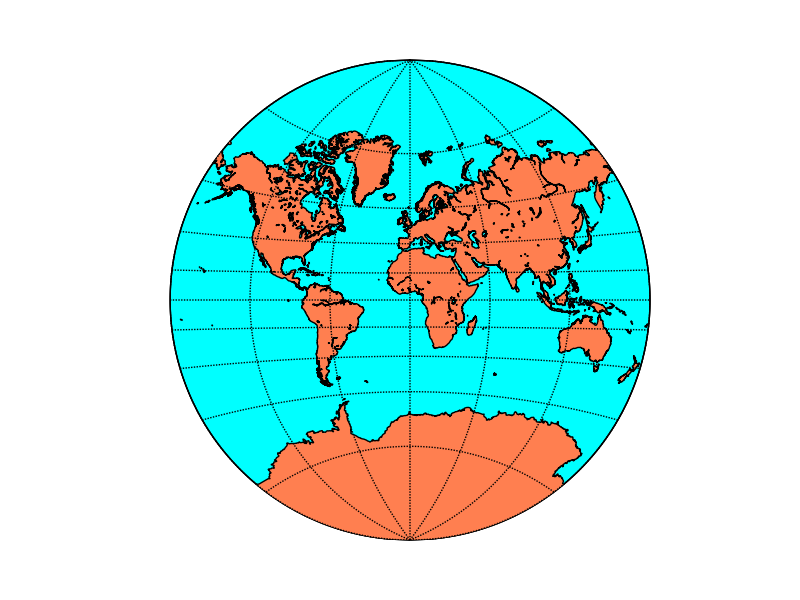
\includegraphics[scale=0.5,origin=c]{/Users/student/seminar/Kartendarstellungen/seminar/vandg} \caption{Van der Grinten Projektion}
\end{figure}
\newpage 